% !TEX program = xelatex
\documentclass[12pt]{article}

% --- HCMUS Report Style Package ---
\usepackage{hcmus-report-template}

% --- Additional Packages for L_RAG System Architecture ---
\usepackage{fontspec}
\usepackage{booktabs}
\usepackage{longtable}
\usepackage{multirow}
\usepackage{titlesec}
\usepackage{tikz}
\usetikzlibrary{shapes.geometric, arrows, positioning}

% Disable indentation on new paragraphs
\setlength{\parindent}{0pt}

% Line spacing 1.2
\renewcommand{\baselinestretch}{1.2}

% --- Course and Report Metadata ---
\newcommand{\coursename}{Text Mining}
\newcommand{\reporttitle}{L\_RAG: Knowledge-Graph-Augmented Hybrid Legal RAG System}
\newcommand{\reportname}{System Architecture, Corpus Design, and Retrieval Components}

\newcommand{\studentname}{\textbf{Tran Tuan Kiet} (23127215) \\ \textbf{Binh}}
\newcommand{\teachername}{Dr. Nguyen Ngoc Thao \\ M.Sc. Huynh Lam Hai Dang \\ B.Sc. Tran Huy Ban}

% --- Header & Footer Configuration ---
\lhead{\reporttitle}
\rhead{
VNUHCM -- University of Science\\
\coursename
}

% ============ DOCUMENT ============
\begin{document}

\pagenumbering{roman}
\begin{titlepage}
\newcommand{\HRule}{\rule{\linewidth}{0.5mm}}
\centering

\textsc{\Large Vietnam National University Ho Chi Minh City}\\[0.4cm]
\textsc{\Large University Of Science}\\[0.4cm]
\textsc{\large Faculty Of Information Technology}\\[0.5cm]

\IfFileExists{img/hcmus-logo.png}{%
  \includegraphics[scale=.25]{img/hcmus-logo.png}\\[0.5cm]%
}{%
  \IfFileExists{hcmus-logo.png}{%
    \includegraphics[scale=.25]{hcmus-logo.png}\\[0.5cm]%
  }{%
    \vspace{0.5cm}%
  }%
}

\HRule \\[0.3cm]
{ 
\huge{\bfseries{\reporttitle}}\\[0.4cm]
\ifdefined\reportname
  \ifx\reportname\empty\else
    \large{\bfseries{\reportname}}\\[0.2cm]
  \fi
\fi
}
\HRule \\[0.4cm]

\textbf{\large Course: \coursename}\\[0.5cm]

\begin{minipage}[t]{0.48\textwidth}
\begin{flushleft} \large
\emph{Students:}\\
\studentname
\end{flushleft}
\end{minipage}
~
\begin{minipage}[t]{0.48\textwidth}
\begin{flushright} \large
\emph{Lecturers:} \\
\teachername
\end{flushright}
\end{minipage}\\[1cm]

\vfill
{\large \today}\\[1cm]

\end{titlepage}


\tableofcontents
\pagebreak

\begin{abstract}
Legal Information Retrieval (IR) and Question Answering (QA) pose significant technical challenges due to domain-specific terminology, complex document hierarchies, temporal validity constraints, and cross-document statutory references. Standard dense retrieval systems often fail to capture exact statutory citations and cross-article dependencies, while traditional keyword search misses semantic paraphrasing. In this work, we introduce \textbf{L\_RAG}, a comprehensive Knowledge-Graph-augmented hybrid RAG architecture designed for Vietnamese legal corpora. The system integrates dual-stage retrieval (Dense \texttt{multilingual-e5-large} + Sparse BM25), Knowledge Graph dynamic overlays for legal validity and structural traversal, Reciprocal Rank Fusion (RRF), multi-reranker candidate refinement (CrossEncoder, BGE-v2, Jina-v2, Qwen3-Reranker), and citation-grounded LLM synthesis. This document presents a complete description of the system architecture, component specifications, knowledge graph schema, and corpus design up to the experimental evaluation setup.
\end{abstract}

\newpage

\pagenumbering{arabic}
\setcounter{page}{1}

% --- System Description Sections (Completed by Kiet) ---
% ============================================================================
% Section 1: Introduction scaffold
% ============================================================================
\section{Introduction}
\label{sec:introduction}

\textit{Guidance: Introduce the Vietnamese legal QA problem, motivate
traceable evidence, and preview the report contributions. Keep this chapter
focused on why the problem matters; reserve implementation details for
Sections~\ref{sec:system-design} and~\ref{sec:implementation-setup}.}

\subsection{Background and Motivation}
\label{sec:intro-motivation}

\textit{Guidance: Add a motivating Vietnamese legal question, the governing
provision, and an explanation of why a cited answer is required. Include the
planned motivation figure and the keyword-search versus vector-RAG versus
L\_RAG contrast.}

\subsection{Problem Statement}
\label{sec:problem-statement}

\textit{Guidance: State the failure modes to be addressed: long documents,
hierarchy blindness, cross-document references, outdated provisions, missing
text, and unsupported answers. Add the problem-to-consequence table.}

\subsection{Project Objectives}
\label{sec:objectives}

\textit{Guidance: List measurable objectives and map each objective to an
implemented module, source file or script, and validation evidence. Add the
contribution map.}

\subsection{Scope of the System}
\label{sec:scope}

\textit{Guidance: Define the included corpus, preprocessing, graph, retrieval,
generation, and evaluation stages. Explicitly list excluded capabilities and
the assumptions that limit deployment.}

\subsection{Main Contributions}
\label{sec:contributions}

\textit{Guidance: Summarize the structured legal corpus, G-LRAG graph,
hybrid retrieval pipeline, citation-grounded generation, and controlled
ablation study. Use one contribution overview figure.}

\subsection{Report Organization}
\label{sec:report-organization}

\textit{Guidance: Explain the Problem $\rightarrow$ Data $\rightarrow$
Methodology $\rightarrow$ Implementation $\rightarrow$ Evaluation
$\rightarrow$ Ablations $\rightarrow$ Discussion $\rightarrow$ Conclusion
flow and add the report-roadmap figure.}

% ============================================================================
% Section 2: Background and Related Work scaffold
% ============================================================================
\section{Background and Related Work}
\label{sec:related-work}

\textit{Guidance: Replace these prompts with a focused literature review.
Explain which prior ideas motivate each L\_RAG design choice and identify the
gap addressed by the controlled ablations.}

\subsection{Retrieval-Augmented Generation}
\label{sec:related-rag}

\textit{Guidance: Define the standard query, retriever, context, prompt, LLM,
and answer pipeline. Add a standard RAG diagram and a grounding illustration.}

\subsection{Legal Information Retrieval}
\label{sec:related-legal-ir}

\textit{Guidance: Discuss authority, hierarchy, temporal validity, citation
dependencies, and the cost of retrieval errors in legal settings. Add the
legal-document hierarchy and a legal retrieval example.}

\subsection{Dense, Sparse, and Hybrid Retrieval}
\label{sec:related-hybrid}

\textit{Guidance: Compare dense retrieval, BM25, and rank fusion. Add the
retrieval comparison table and a vocabulary-mismatch example.}

\subsection{Knowledge-Graph-Augmented Retrieval}
\label{sec:related-graph}

\textit{Guidance: Explain how graph structure supplies containment,
neighboring, citation, amendment, and validity context. Add a graph-retrieval
illustration and a vector-versus-graph comparison table.}

\subsection{Reranking and Citation-Grounded Generation}
\label{sec:related-reranking}

\textit{Guidance: Introduce candidate reranking, cross-encoders, citation
grounding, and abstention. Add the two-stage ranking and citation-grounding
illustrations.}

\subsection{Design Requirements for Legal RAG}
\label{sec:related-requirements}

\textit{Guidance: Convert legal reliability requirements into design choices
and evaluation checks. Add a requirement traceability matrix and design
rationale diagram.}

% ============================================================================
% Section 3: Legal Dataset and Benchmark Construction scaffold
% ============================================================================
\section{Legal Dataset and Benchmark Construction}
\label{sec:dataset-construction}

\textit{Guidance: Describe the corpus and benchmark as reproducible data
products. Keep the running Vietnamese legal question consistent across the
dataset, graph, retrieval, and generation examples.}

\subsection{Legal Corpus and Raw Data Sources}
\label{sec:raw-corpus}

\textit{Guidance: Inventory raw files, record types, identifiers,
relationships, and text fields. Reuse the document-type distribution and add
a sanitized metadata and relationship example.}

\subsection{Dataset Normalization and Cleaning}
\label{sec:dataset-normalization}

\textit{Guidance: Document identifier, date, document-type, status, and
relationship transformations. Reuse the data-pipeline figure and add a
before-and-after record plus a normalization-rules table.}

\subsection{Relationship Processing and External References}
\label{sec:relationship-processing}

\textit{Guidance: Explain resolved in-corpus targets, unresolved external
targets, external stubs, relationship vocabulary, and direction verification.
Add the relationship-resolution diagram, vocabulary table, and stub example.}

\subsection{Quarantine and Data-Quality Verification}
\label{sec:quarantine}

\textit{Guidance: Show accepted records, quarantined records, verification
gates, final inclusion, audit counts, and reconciliation identities. Reuse the
edge-quarantine asset.}

\subsection{Legal Text Structuring}
\label{sec:text-structuring}

\textit{Guidance: Describe the Document $\rightarrow$ Provision $\rightarrow$
Chunk hierarchy and provenance pointers. Reuse the provision and chunk assets
and add the structured-artifact inventory.}

\subsection{QA Benchmark Construction}
\label{sec:benchmark-construction}

\textit{Guidance: Show context sampling, question generation, verification,
diversity filtering, deduplication, and final export. Add the benchmark-flow
figure, a record example, and stage-count table.}

\subsection{Question Categories and Answer Types}
\label{sec:question-taxonomy}

\textit{Guidance: Define single-hop, citation, legal-validity, multi-hop, and
cross-document categories, and relate them to abstractive, boolean,
extractive, and unanswerable answer types. Add the category-answer-type
matrix.}

\subsection{Ground-Truth Evidence}
\label{sec:ground-truth}

\textit{Guidance: Explain reference answers and document, provision, and chunk
identifiers. Add the evidence-link diagram, annotated JSONL record, and
ground-truth coverage table.}

\subsection{Dataset Statistics and Validation}
\label{sec:dataset-validation}

\textit{Guidance: Report corpus size, missing-text counts, orphan counts,
quarantine counts, external stubs, and reconciliation checks. Reuse the
length, node-type, and document-type assets and add a validation dashboard.}

% ============================================================================
% Section 4: L_RAG System Design and Methodology
% ============================================================================
\section{L\_RAG System Design and Methodology}
\label{sec:system-design}

L\_RAG turns the structured corpus and benchmark into an evidence-oriented
retrieval and generation pipeline. Offline processing creates normalized
records, graph artifacts, and vector or sparse indexes. Online processing
resolves query scope, retrieves candidate chunks, optionally expands or
filters them with the graph, reranks a bounded pool, and serializes the final
context for a citation-grounded generator. The same document, provision, and
chunk identifiers introduced in Section~\ref{sec:dataset-construction} are
carried through every stage.

\subsection{End-to-End System Architecture}
\label{sec:architecture}

The architecture has five operational phases: (1) query and temporal-scope
resolution, (2) dense and optional sparse retrieval, (3) graph filtering or
context expansion, (4) rank fusion and candidate reranking, and (5) prompt
construction, generation, and cited output. \hyperref[fig:architecture]{Figure~\ref*{fig:architecture}}
shows the data flow and the point at which each family of ablations changes a
component.

\begin{figure*}[t]
\centering
\resizebox{\textwidth}{!}{%
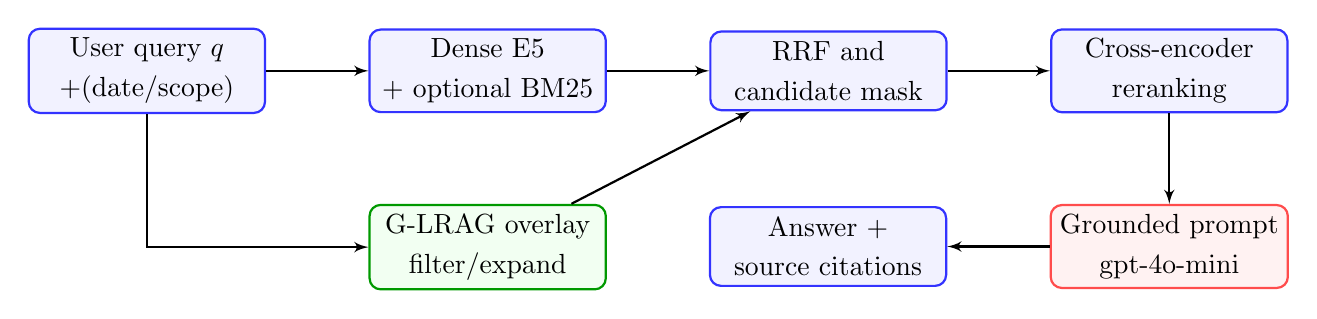
\begin{tikzpicture}[node distance=1.45cm, auto,
    block/.style={rectangle, draw=blue!80, fill=blue!5, thick, minimum width=3cm, minimum height=1cm, align=center, rounded corners},
    kgblock/.style={rectangle, draw=green!60!black, fill=green!5, thick, minimum width=3cm, minimum height=1cm, align=center, rounded corners},
    llmblock/.style={rectangle, draw=red!70, fill=red!5, thick, minimum width=3cm, minimum height=1cm, align=center, rounded corners},
    line/.style={draw, -latex', thick}]
    \node [block] (query) {User query $q$\\+(date/scope)};
    \node [block, right=1.3cm of query] (retrieve) {Dense E5\\+ optional BM25};
    \node [kgblock, below=1.15cm of retrieve] (graph) {G-LRAG overlay\\filter/expand};
    \node [block, right=1.3cm of retrieve] (fuse) {RRF and\\candidate mask};
    \node [block, right=1.3cm of fuse] (rank) {Cross-encoder\\reranking};
    \node [llmblock, below=1.15cm of rank] (generate) {Grounded prompt\\gpt-4o-mini};
    \node [block, left=1.3cm of generate] (output) {Answer +\\source citations};
    \path [line] (query) -- (retrieve);
    \path [line] (query) |- (graph);
    \path [line] (retrieve) -- (fuse);
    \path [line] (graph) -- (fuse);
    \path [line] (fuse) -- (rank);
    \path [line] (rank) -- (generate);
    \path [line] (generate) -- (output);
\end{tikzpicture}%
}%
\caption{End-to-end operational workflow of L\_RAG. The graph and reranker
stages are optional branches whose effects are tested under separate frozen
ablation controls.}
\label{fig:architecture}
\end{figure*}

The component boundaries are deliberate. The retriever decides which chunks
are available, the graph can alter that set under a fixed context budget, the
reranker only reorders a candidate pool, and the generator sees a serialized
top-10 context. This separation prevents a generation metric from being
mistaken for evidence-retrieval quality.

\subsection{Offline Data and Index Construction}
\label{sec:offline-construction}

Offline construction branches from the normalized records into three linked
artifacts. The structured-text branch emits provisions and chunks with stable
parent pointers. The graph branch emits document, provision, chunk, and
relationship nodes plus validity and authority metadata. The retrieval branch
embeds either chunk-only or header-plus-chunk text into a FAISS index and
builds tokenized BM25 shards for configurations that enable sparse retrieval.

The dense index uses L2-normalized vectors and inner-product search, which is
equivalent to cosine ranking for normalized embeddings. For the completed
hybrid runs, BM25 is built as 10 independent shards with shard-local IDF and
average-document-length statistics; shard candidates are merged by BM25 score
before RRF. The graph and index artifacts keep the same chunk IDs, so a
retrieved vector row can be joined back to its document and provision without
fuzzy matching. Frozen manifests record the corpus snapshot, model
checkpoint, index path, configuration name, and benchmark version used to
create each evaluation run.

\subsection{Online Query-Processing Workflow}
\label{sec:online-query}

At query time, the system first preserves the raw Vietnamese question and any
explicit date or scope constraint. The query encoder produces an E5 vector;
the dense branch retrieves a broad seed set, while the optional BM25 branch
searches tokenized shards. The branches are merged with RRF when hybrid mode
is enabled. In the completed retrieval/graph family, a graph variant keeps
the top five seeds, expands them within their parent provisions with
\texttt{max\_hop=1}, and replaces the baseline top-10 context with at most
ten expanded chunks. This is a complete context-selection policy: it uses
broad validity filtering and does not apply a query-time validity overlay or
reranking. The resulting candidates are trimmed to the family-specific
budget, reranked only in the reranker family, and serialized as the final
context.

Insufficient evidence follows an observable fallback path. If no candidate
survives a valid scope filter, if the context contains no usable text, or if
the prompt's evidence threshold is not met, the retrieval/graph prompt asks
the model to emit the Vietnamese fallback phrase
\textit{``Không có đủ thông tin trong ngữ cảnh được cung cấp.''}; the
fixed-context reasoning runs use the visible marker
\texttt{INSUFFICIENT\_CONTEXT}. These strings are saved for evaluation and
are not treated as proof that a question was legally unanswerable. Invalid
filters and unresolved external references remain visible in the run record
instead of being silently repaired.

\subsection{Knowledge Graph Construction}
\label{sec:graph-construction}

The G-LRAG graph uses Document ($D$), Provision ($P$), Chunk ($C$), and
ExternalStub nodes. Structural edges encode
\texttt{DOCUMENT\_HAS\_PROVISION}, \texttt{PROVISION\_HAS\_CHUNK},
\texttt{CHUNK\_NEXT}, and \texttt{PROVISION\_NEXT}. Legal-relation edges encode
citations, amendments, replacements, and repeals. Each edge retains source
provenance and is available to query-time traversal only after direction and
endpoint checks.

The overlay can fold validity fields relative to an \texttt{as\_of\_date}
parameter and can sort candidates by authority rank. A simplified precedence
ordering available to the system is
\begin{equation}
\text{Constitution} \succ \text{Law/Code} \succ
\text{Decree} \succ \text{Circular}.
\end{equation}
Reading-order traversal follows adjacent chunks or provisions to recover
nearby context; hop 1 covers the seed provision and additional hops reach
subsequent provisions. In the completed graph ablation, traversal is limited
to five seeds and at most ten retained chunks, with no query-time validity
overlay or reranking. This policy can replace strong seed evidence and is
therefore evaluated as a change to the candidate set, not as a free context
addition.

\subsection{Retrieval and Ranking}
\label{sec:retrieval-ranking}

The dense encoder is \texttt{intfloat/multilingual-e5-large}. For the
metadata condition, the indexed string is
\begin{equation}
\begin{aligned}
\text{Text}_{\mathrm{embed}}={}&\text{DocumentTitle}
\;\parallel\;\text{ProvisionHeader}\\
&\;\parallel\;\text{ChunkContent}.
\end{aligned}
\end{equation}
the chunk-only condition removes the first two fields. The FAISS index uses
\texttt{IndexFlatIP}. Sparse retrieval uses \texttt{rank\_bm25} with
\texttt{underthesea} tokenization and $k_1=1.5$, $b=0.75$. Dense and sparse
lists are fused by
\begin{equation}
\mathrm{RRF}(d)=\sum_{m\in\{\mathrm{dense},\mathrm{BM25}\}}
\frac{1}{60+r_m(d)}.
\end{equation}

The dense/hybrid/graph family retrieves 50 seeds and retains at most ten final
chunks. The reranker family reconstructs a common RRF pool of 30 candidates
($C_{30}$), then retains ten ($T_{10}$). mMiniLM, Qwen3, BGE, and Jina score
the full query--candidate pair with a cross-encoder. Models are loaded,
executed, and unloaded sequentially to avoid GPU memory interference. The
reranker can improve ordering inside $C_{30}$, but it cannot recover evidence
that never entered the pool.

\subsection{Answer Generation}
\label{sec:answer-generation}

The context serializer writes each retained chunk with its chunk ID, document
title, provision header, and passage text. All generators use temperature
$0.0$, but output limits are family-specific: the retrieval/graph runs set no
explicit client-side token cap, while the fixed-context reasoning comparison
uses a 1,024-token limit. The retrieval/graph prompt asks for Vietnamese
answers and uses the fallback phrase
\textit{``Không có đủ thông tin trong ngữ cảnh được cung cấp.''} when the
evidence is insufficient; the reasoning runs use the visible marker
\texttt{INSUFFICIENT\_CONTEXT}. A citation should identify the governing
article or instrument.

The observable output record contains the final answer, citation markers,
parser fields, refusal marker, latency, and the ordered context IDs. It does
not contain hidden chain-of-thought, reasoning-token accounting, or a human
claim-entailment annotation. Consequently, the evaluation can report output
format and lexical overlap but cannot infer legal correctness from a fluent
answer or a well-formed citation.

\subsection{End-to-End Worked Example}
\label{sec:worked-example}

Consider a benchmark question asking whether a specified land-use action is
permitted under a named Vietnamese instrument. The source record is first
joined to its document ID and effective date. Its controlling article is
represented as a provision, and the provision is split into ordered chunks
whose IDs remain linked to the parent. The query encoder retrieves candidate
chunks; the graph can add the adjacent clause or a cited instrument; RRF and
the reranker order the retained candidates; and the serializer presents the
top ten with their provenance.

The generator then produces an answer in the requested format and attaches
the document and provision identifiers used as citations. If the retrieved
context contains only a related definition but not the operative condition,
the intended output is \texttt{INSUFFICIENT\_CONTEXT}. The example illustrates
why the report distinguishes document success from exact chunk recall and
citation presence from citation entailment: each is a different observable
stage in the same traceable workflow.


% ============================================================================
% --- Future Evaluation & Results Sections (To be filled by Binh) ---
% % ==========================================================================
% Section 5: Implementation and Experimental Setup
% ==========================================================================
\section{Implementation and Experimental Setup}
\label{sec:implementation-setup}

This section states the controls and scoring rules needed to interpret the
ablations in Section~\ref{sec:ablation-study}. The experiment families share
a benchmark but are not a single factorial experiment: candidate pools,
context construction, and latency accounting differ. Variants are therefore
compared only within their own controlled family.

\subsection{Pipeline and Frozen Artifacts}
\label{sec:software-architecture}

The evaluated pipeline has five stages: query embedding with
\texttt{intfloat/multilingual-e5-large}; dense FAISS retrieval and, where
enabled, tokenized BM25 retrieval; RRF fusion, graph expansion, or
cross-encoder reranking; serialization of retained chunks into a grounded
prompt; and answer generation and evaluation. The analysis reads frozen
manifests, predictions, aggregate metrics, latency records, and error logs;
it does not rerun models. Every primary comparison is joined by
\texttt{qa\_id}, so an aggregate difference is traceable to paired cases.

\subsection{Indexes, Graph, and Runtime Settings}
\label{sec:build-process}

The dense/hybrid/graph experiment uses a FAISS index with 1,513,376 chunk
vectors and a graph over the same number of chunks. The hybrid branch searches
ten BM25 shards. Dense/hybrid retrieval uses a 50-result search budget, broad
filtering, a final context of 10 chunks, and RRF parameter $k=60$ where BM25
is enabled. Graph variants take five seeds, traverse one hop, and retain at
most 10 graph-context chunks. The dense/hybrid and reranker generation
artifacts use GPT-4o-mini.

The reranker family fixes a 30-chunk RRF candidate pool (C30) and a 10-chunk
final context (T10), comparing no reranking, RRF-only, mMiniLM, Qwen3, BGE,
and Jina. The primary generator study compares GPT-4o-mini Base and CoT with
the saved top-10 context fixed by question. The metadata study changes only
the indexed string from chunk body to header-plus-chunk text; encoder, FAISS,
top-$k=10$, generator, prompt, seed, corpus, and benchmark stay fixed.

\subsection{Benchmark and Metrics}
\label{sec:evaluation-metrics}

The benchmark contains 500 questions: 400 answerable questions with gold
chunk identifiers and 100 unanswerable questions. Retrieval scores use only
the 400 answerable records. Given gold chunks $G$ and retrieved top-$k$ chunks
$R_k$, context recall is $|G \cap R_k|/|G|$; Hit@k indicates that at least one
gold chunk occurs. MRR and nDCG reward early gold rank. Candidate Recall@30 is
the evidence ceiling for the reranker study and is intentionally identical
for every reranker.

Exact Match, Token F1, and ROUGE-L are lexical overlap with reference answers.
The saved unanswerable score is a refusal-marker diagnostic, not a semantic
assessment of legal appropriateness. Citation presence and structural coverage
measure saved marker/parser fields, not claim-to-source entailment. Latency is
reported as saved p50/p95 timing; cached-BM25 reranker timing is not full
online sparse-retrieval timing.

\subsection{Pairing, Uncertainty, and Claim Boundaries}
\label{sec:experimental-protocol}

Headline effects are paired by \texttt{qa\_id}. Retrieval uses the shared
answerable intersection; scheduled-denominator answerability diagnostics keep
all 500 cases. Percentile paired-bootstrap confidence intervals use 10,000
resamples for headline metadata, dense/hybrid, reranker, and GPT comparisons;
reranker slices use 2,000. Intervals crossing zero are reported as
inconclusive. The non-GPT prompt pairs are descriptive when code provenance,
timeouts, retries, or retrieved context differ.

No blinded legal-correctness labels, claim-level faithfulness labels, or
validated semantic judge are available. Thus, no result is interpreted as
proof of legal correctness, legal safety, citation entailment, or faithful
reasoning merely because it improves a lexical, rank, citation-format, or
refusal-format metric.

% \input{sections/6_results}
% \input{sections/7_discussion}
% \input{sections/8_conclusion}
% ============================================================================

\end{document}
